
\begin{bt}%[0D7N1-2]%[Dự án đề kiểm tra Toán 10 GHKII NH23-24- Trần Xuân Hòa]%[THPT Trường Chinh]
Giài bất phương trình $x^2-4>0$.
\loigiai{Đặt $VT=x^2-4$. Ta có $VT=0\Rightarrow x=\pm 2$. Ta có bảng xét dấu
\begin{center}

\begin{tikzpicture}
	\tkzTabInit[deltacl=0.5,espcl=2.5,lgt=2]
	{$x$/1,$VT$/1}
	{$-\infty$,$-2$,$2$,$+\infty$}
	\tkzTabLine{,+,z,-,z,+,}
\end{tikzpicture}
	\end{center}
Từ bảng xét dấu, bất phương trình có tập nghiệm $S=(-\infty ; 2)\cup (2; +\infty)$.
}
\end{bt}
%Câu 2...........................
\begin{bt}%[0D7H1-2]%[Dự án đề kiểm tra Toán 10 GHKII NH23-24- Trần Xuân Hòa]%[THPT Trường Chinh]
Tìm tất cả các giá trị của tham số $m$ để $2 x^2-2(3 m+1) x+3 m+5>0$ có nghiệm đúng với mọi số thực $x$.
	\loigiai{Ta có $a=2>0$; $\Delta =36(m^2-1)$.\\
	Bất phương trình có nghiệm với $\forall x\in \mathbb{R}$ khi và chỉ khi 
	\begin{eqnarray*}
		&&\heva{&a>0\\ &\Delta <0}\\
		&\Rightarrow&36(m^2-1)<0\\
		&\Rightarrow&-1<m<1.
	\end{eqnarray*}
Vậy các giá trị $m$ cần tìm là $m\in (-1;1)$.
	}
\end{bt}
%Câu 3...........................
\begin{bt}%[0D7N3-2]%[Dự án đề kiểm tra Toán 10 GHKII NH23-24- Trần Xuân Hòa]%[THPT Trường Chinh]
Giải phương trình $\sqrt{3 x^2+x+4}=2-x$.	
	\loigiai{
	\begin{itemize}
		\item Bình phương hai vế được $3x^2+x+4=(2-x)^2\Rightarrow 2x^2+5x=0\Rightarrow \hoac{&x=0\\ &x=-\dfrac{5}{2}}$.
		\item Thử lại, thay $x=0$; $x=-\dfrac{5}{2}$ vào phương trình đầu, đều thỏa mãn.
	\end{itemize}
	Vậy nghiệm của phương trình là $S=\left\{-\dfrac{5}{2};0\right\}$.
	}
\end{bt}
%Câu 4...........................
\begin{bt}%[0D7N1-5]%[Dự án đề kiểm tra Toán 10 GHKII NH23-24- Trần Xuân Hòa]%[THPT Trường Chinh]
Lợi nhuận thu được từ việc sản xuất và bán $x$ sản phẩm thủ công của một cửa hàng là $P(x)=-0{,}1 x^2+200 x-51000$ (đơn vị tính bằng nghìn đồng). Với số lượng sản phẩm bán ra là bao nhiêu thì cửa hàng có lăi?	
	\loigiai{
	Cửa hàng có lãi khi $P(x)=-0{,}1 x^2+200 x-51000>0$. \\
	Ta có $P(x)=0\Rightarrow x=300$; $ x=1\;700$. Bảng xét dấu
	\begin{center}
		\begin{tikzpicture}
			\tkzTabInit[deltacl=0.5,espcl=2.5,lgt=2]
			{$x$/1,$P(x)$/1}
			{$-\infty$,$300$,$1700$,$+\infty$}
			\tkzTabLine{,-,z,+,z,-,}
		\end{tikzpicture}
	\end{center}
	Từ bảng xét dấu, $P(x)>0\Rightarrow 300<x<1\;700$.\\
	Vậy với số lượng sản phẩm bán ra trong khoảng $(300;1\;700)$ thì cửa hàng có lãi.
	}
\end{bt}
%Câu 5...........................
\begin{bt}%[0D8N1-2]%[Dự án đề kiểm tra Toán 10 GHKII NH23-24- Trần Xuân Hòa]%[THPT Trường Chinh]
Một bó hoa có $5$ hoa hồng trắng, $6$ hoa hồng đỏ và $7$ hoa hồng vàng. Hỏi có mấy cách chọn lấy ba bông hoa có đủ cả ba màu?	
	\loigiai{
		Lấy được ba bông hoa có đủ ba màu khi thực hiện liên tiếp ba hành động sau
	\begin{itemize}
		\item HĐ1: Lấy được $1$ hoa hồng trắng có $5$ cách.
		\item HĐ2: Lấy được $1$ hoa hồng đỏ có $6$ cách.
		\item HĐ3: Lấy được $1$ hoa hồng vàng có $7$ cách.
	\end{itemize}
	Theo quy tắc nhân, ta có $5\cdot 6\cdot 7=210$ (cách) lấy được $3$ bông hoa có đủ cả ba màu.
	}
\end{bt}
% Câu 6 ..............
\begin{bt}%[0H9N2-1]%[Dự án đề kiểm tra Toán 10 GHKII NH23-24- Phạm Quốc Toàn]%[THPT Trường Chinh]
\begin{enumerate}[a) ] 
\item Cho $\overrightarrow{a} = \left(1; 3 \right)$, $\overrightarrow{b} = \left(6; -2\right)$. Tìm $\overrightarrow{y}$ thỏa mãn $\heva{& \overrightarrow{a} \cdot \overrightarrow{y} =23 \\ & \overrightarrow{b} \cdot \overrightarrow{y} =24}$. 
\item Cho $A \left(1; -2\right)$, $B \left(0; 4\right)$. Tìm tọa độ điểm $E$ trên trục $O x$ sao cho $E$, $A$, $B$ thẳng hàng. 
\end{enumerate}
\loigiai{
\begin{enumerate}[a) ] 
\item Đặt $\overrightarrow{y} = \left(x_0; y_0 \right)$. \\
Theo đề bài ta có $\heva{& \overrightarrow{a} \cdot \overrightarrow{y} =23 \\ & \overrightarrow{b} \cdot \overrightarrow{y} =24} \Leftrightarrow \heva{& x_0 + 3 y_0 =23 \\ & 6 x_0 - 2 y_0 =24} \Leftrightarrow \heva{& x_0 = \dfrac{59}{10} \\ & y_0 = \dfrac{57}{10}}$. \\
Vậy $\overrightarrow{y} = \left(\dfrac{59}{10}; \dfrac{57}{10}\right)$.  
\item Gọi $E \left(x; 0\right)$. \\
Ta có $\overrightarrow{AE} = \left(x-1; 2\right)$, $\overrightarrow{AB} = \left(-1; 6\right)$. \\
$E$, $A$, $B$ thẳng hàng khi và chỉ khi $\overrightarrow{AE} = k \cdot \overrightarrow{AB} \Leftrightarrow \heva{& x-1 = k \cdot (-1) \\ & 2 = k \cdot 6} \Leftrightarrow \heva{& k = \dfrac{1}{3} \\ & x= \dfrac{2}{3}}$. \\ 
Vậy $E \left(\dfrac{2}{3}; 0\right)$. 
\end{enumerate}
}
\end{bt}
% Câu 7 .............
\begin{bt}%[0H9H3-5]%[Dự án đề kiểm tra Toán 10 GHKII NH23-24- Phạm Quốc Toàn]%[THPT Trường Chinh]
Trong mặt phẳng với hệ trục tọa độ $O x y$. 
\begin{enumerate}[a) ] 
\item Viết phương trình tham số của đường thẳng $d$ biết $d$ đi qua điểm $E \left(3; -4\right)$ và có hệ số góc $k=5$. 
\item Tính khoảng cách từ điểm $I \left(-3; 2\right)$ đến đường thẳng $\Delta \colon 4x-3y-7=0$. 
\end{enumerate}
\loigiai{
\begin{enumerate}[a) ] 
\item Phương trình đường thẳng $d$ là $y= 5 \cdot (x-3) + \left(-4 \right) \Leftrightarrow y = 5x -19$. \\
Suy ra phương trình tham số của đường thẳng $d$ là $\heva{& x = t \\ & y = -19 + 5t}$. 
\item Khoảng cách từ điểm $I \left(-3; 2\right)$ đến đường thẳng $\Delta$ là $\mathrm{\,d} \left(I, \Delta \right) = \dfrac{|4 \cdot \left(-3 \right) -3 \cdot 2 -7|}{\sqrt{4^2 + \left(-3 \right)^2}} = 5$.  
\end{enumerate}
}
\end{bt}
% Câu 8 .............
\begin{bt}%[0H9H2-1]%[Dự án đề kiểm tra Toán 10 GHKII NH23-24- Phạm Quốc Toàn]%[THPT Trường Chinh]
Trong mặt phẳng $O x y$, cho điểm $A \left(1; 4\right)$. Gọi $B$ là điểm đối xứng với $A$ qua gốc tọa độ $O$. Tìm tọa độ điểm $C$ sao cho tam giác $ABC$ vuông cân tại $C$. 
\loigiai{
$B$ là điểm đối xứng với $A$ qua gốc tọa độ $O$, suy ra $B \left(-1; -4 \right)$. \\
Gọi $C \left(x; y\right)$. Ta có $\overrightarrow{AC} = \left(x-1; y-4\right)$, $\overrightarrow{BC} = \left(x+1; y+4\right)$. \\
Tam giác $ABC$ vuông cân tại $C \Leftrightarrow \heva{& \overrightarrow{AC} \cdot \overrightarrow{BC} = 0 \\ & AC = BC} \Leftrightarrow \heva{& \left(x^2 -1 \right) + \left(y^2 - 16 \right) = 0 \\ & \left(x-1 \right)^2 + \left(y-4 \right)^2 = \left(x+1 \right)^2 + \left(y+4 \right)^2}$ \\
$\Leftrightarrow \heva{& x^2 +y^2 =17 \\ & x + 4y =0} \Leftrightarrow \heva{& x = - 4y \\ & 17 y^2 = 17} \Rightarrow \heva{& x=-4 \\ & y=1}$ hoặc $\heva{& x=4 \\ & y=-1}$. \\
Vậy có hai điểm thỏa mãn là $C \left(-4; 1 \right)$ hoặc $C \left(4; -1 \right)$.
}
\end{bt}
%%%%%%%%%%%%%%%%%%%%%%%%%%%%%%%%%%%%%%%%%%%%%